%\usepackage [ISO-8859-1]{inputenc}
\documentclass[a4paper,12pt,oneside]{amsbook}
\usepackage[T1]{fontenc}
\usepackage{listings}
\usepackage{textcomp}
\usepackage{multicol}
%\usepackage{euler}
%\usepackage{garamond}
\usepackage{hyperref}

\usepackage{newcent}
%\fontfamily{fxm}\selectfont
\usepackage{fancyhdr}
\pagestyle{fancy}
% Detta paket skoter grafiken
%\usepackage[dvips]{graphicx}
\usepackage[pdftex]{graphicx}

\usepackage{amsthm}
\usepackage{amsmath}
\usepackage[swedish]{babel}
% For bortkommentering
\usepackage{verbatim}
% For att slippa indentering av Sections och SubSections
\usepackage{indentfirst}

% Har stalls paragrafindentering och avstand mellan stycken och rader mm
\setlength{\parindent}{0pt}
\setlength{\parskip}{6pt}
\setlength{\baselineskip}{12pt}
% Har definieras sidan
\setlength{\voffset}{-15mm}
\setlength{\hoffset}{-5.5mm}

\setlength{\topmargin}{0mm}
\setlength{\headheight}{10mm}
\setlength{\headsep}{8mm}
\setlength{\footskip}{16mm}

\setlength{\evensidemargin}{0mm}
\setlength{\oddsidemargin}{0mm}

\setlength{\marginparsep}{0mm}
\setlength{\marginparwidth}{0mm}

\setlength{\textwidth}{170mm}
\setlength{\textheight}{230mm}
\setlength{\paperwidth}{210mm}
\setlength{\paperheight}{297mm}
\setlength{\headwidth}{170mm}
% Huvud och Fot
%\fancypagestyle{}{
\fancyhf{}\fancyhead[c]{\small{\textit{Programmeringsolympiaden Kvalificering 2022}}}
\fancyfoot[c]{\thepage}
\renewcommand{\headrulewidth}{0.4pt}
\renewcommand{\footrulewidth}{0.4pt}
\newenvironment{lista}
{\begin{itemize}
\setlength{\parindent}{0pt}
\setlength{\itemsep}{6pt}}
{\end{itemize}}
% Uppgifter
\newcounter{probnr}
\newenvironment{tal}{%
\begin{list}
%{\textbf{\arabic{section}.\arabic{probnr}}} {\usecounter{probnr}
{\textbf{\arabic{probnr}}} {\usecounter{probnr}
\setlength{\leftmargin}{0mm}
\setlength{\rightmargin}{0mm}
\setlength{\labelwidth}{-1mm}
\setlength{\labelsep}{1mm}}
\setlength{\itemsep}{6pt}
}{\end{list}}
% Definition av avsnitt: FAKTA, EXEMPEL, PASTAENDE
\newtheorem{fakta}{Fakta}
\newtheorem{exempel}{Exempel}
\newtheorem{problem}{Problem}
%
\newtheoremstyle{test}% NAME
{20pt}      % ABOVESPACE
{10pt}      % BELOWSPACE
{\sffamily} % BODYFONT
{0pt}       % INDENT
{\scshape}  % HEADFONT
{}          % HEADPUNCT
{\newline}  % HEADSPACE
{}          % CUSTOM-HEAD-SPEC

\theoremstyle{test}
\newtheorem{program}{Program}
\newcommand{\sv}[1]{\textsc{#1}}            % Sma versaler
\newcommand{\fe}[1]{\textbf{#1}}            % FET
\newcommand{\ku}[1]{\textit{#1}}            % KURSIV
\newcommand{\cu}[1]{\texttt{#1}}            % Courier
\newcommand{\sk}[1]{\texttt{#1}}            % Courier
\newcommand{\rubrik}[1]{\begin{center}\sf\huge{#1}\normalsize\rm\end{center}}
\begin{document}
%\DeclareGraphicsExtensions{.jpg,.pdf,.mps,.png,.eps}


\thispagestyle{fancy}
\lstset{basicstyle=\ttfamily,
  breaklines=true}
% ----------------------------------------------------

\begin{center}
\Huge{Programmeringsolympiaden 2022}
\end{center}
\vspace{-1.2cm} 
\specialsection*{Tävlingsregler för skolkvalet}
\begin{lista}
\item Tävlingen äger rum på av skolan bestämt datum under {\bf fyra
    timmar. Ingen förlängning ges för lunch eller raster.} Eleven ska i förväg komma överens med läraren om att använda egen dator eller en som skolan tillhandahåller. I vilket fall som helst måste eleven befinna sig i avtalad lokal på skolan. {\bf På grund av pandemin kan i undantagsfall tävling ske från annan plats godkänd av läraren, givet tillräcklig övervakning}
\item Tävlingen består av sex uppgifter som vardera ska lösas genom ett
  datorprogram i valfritt programmeringsspråk.
\item {\bf Indata kan läsas in i programmet på valfritt sätt}, t.ex. genom att programmet för en dialog med användaren (som i körningsexemplena i uppgifterna), att de skrivs in i ett grafiskt gränssnitt eller att datafiler skickas till {\em standard input}. Kom bara överens med din lärare om hur programmet ska testas.
\item Dina lösningar kommer att testköras med förpreparerade
  indata. Varje uppgift testas normalt med 5 testfall, som vardera ger
  1 poäng om ditt program skriver ut korrekt svar inom en exekveringstidsgräns av
  {\bf 3 sekunder}. Ingen test av indata behöver göras, den följer specifikationerna 
i uppgiften.
\item Det är ofta olika begränsningar på de olika testfallen, t.ex.\ storleken på
indata eller andra inskränkningar. Detta anges i uppgiften. {\bf Observera att det kan vara
helt olika svårighetsgrad på en uppgift beroende på dessa skillnader. Det kan därför vara
lättare att få delpoäng på en uppgift som verkar svår än att få full
poäng på en uppgift som verkar lättare.} Informationen om delpoäng är
därför extremt viktig för att planera sin
tävling.
\item Rättningen utförs på samma eller likvärdig dator. Ändringar
  i källkoden tillåts ej efter tävlingen. Om programmet
  inte kan kompileras ges 0 p.\ på uppgiften. 
\item Om något av följande inträffar ger
  det {\em testfallet} 0 poäng, men programmet fortsätter testas med övriga testfall.
\begin{lista}
\item Exekveringstiden överstiger 3 sekunder \vspace{-0.2cm}
\item Exekveringsfel (run time error) \vspace{-0.2cm}
\item Fel svar \vspace{-0.2cm}
\end{lista}

\item Deltagandet är individuellt vilket bland annat innebär att inget utbyte av idéer eller 
filer får ske under tävlingen.  
\item Hjälpmedel: Valfritt skriftligt material, material som finns installerat på datorn samt material som finns tillgängligt på internet. Det är \ku{inte} tillåtet att aktivt kommunicera på internet (t.ex. chatta eller ställa frågor till ett forum) utan endast att söka efter information. Räknedosa är tillåten.
\item Tävlingsbidraget ska lämnas in i form av källkodsfiler (uppg1...uppg6 med passande filtillägg) som läggs på överenskommen plats. Ingen hänsyn tas till andra filer. Var noga 
med att lämna in den korrekta versionen av ditt program.  
\end{lista}

%De högst placerade i kvalet går vidare till finalen där landslagsplatser till BOI i Sverige och IOI i Japan står på spel.
\begin{center}
\Large Lycka till!
\end{center}
%\end{document}

\newpage
\specialsection*{Uppgift 1 -- Affischutskicket}

VE OCH FASA!
PostNord har för det $1337$:e året i rad höjt portot, vilket riskerar att bräcka Programmeringsolympiadens budget.

Varje år skickar PO ut affischer till ca $450$ gymnasieskolor. Ett utskick består av tre saker: 
\begin{itemize}
\item ett kuvert av C4-storlek ($229\text{ mm} \times 324\text{ mm}$)
\item två affischer av A3-storlek ($297\text{ mm} \times 420\text{ mm}$)
\item ett informationsblad av A4-storlek ($210\text{ mm} \times 297\text{ mm}$)
\end{itemize}

Det är mycket viktigt att brevet väger högst $50$ gram, eftersom portot annars blir dubbelt så högt. För att klara denna magiska viktgräns kan PO kontrollera tre faktorer: pappersvikten på kuvertet, affischerna och informationsbladet. Pappersvikt anges typiskt i $\frac{\text{gram}}{\text{m}^2}$, där dimensionerna framgår ovan. Notera att kuvertet består av \textbf{två sammanklistrade ark} av C4-storlek, medan pappersvikter och mått är för \emph{ett ark}.

Skriv ett program som givet ett förslag på pappersvikt för kuvert, affisch och informationsblad, räknar ut den totala vikten för brevet.

Programmet ska läsa in tre heltal mellan $50$ och $200$, pappersvikterna i $\frac{\text{gram}}{\text{m}^2}$ för kuvertet, affischerna och informationsbladet. Skriv ut ett enda decimaltal: vikten på ett fullständigt brevutskick i gram. Svaret ska anges med minst $6$ decimalers noggrannhet (d.v.s. vara inom $5 \cdot 10^{-7}$ från rätt svar).

%Svaret kommer alltid att ha högst $6$ siffror efter decimaltecknet.

\vspace{1cm}

\fe{Körningsexempel 1}
\begin{verbatim}
Kuvert ? 120
Affisch ? 90
Blad ? 70

Svar: 44.626140
\end{verbatim}

\vspace{1cm}

\fe{Körningsexempel 2}
\begin{verbatim}
Kuvert ? 150
Affisch ? 200
Blad ? 90

Svar: 77.768100
\end{verbatim}



\newpage
\specialsection*{Uppgift 2 -- Arabiska}

Det är ganska känt att när man skriver text på arabiska skriver man från höger till vänster.
Det är däremot mindre välkänt att man aldrig skriver ut korta vokaler.

Med vokaler menar vi en av bokstäverna: \textit{a,e,i,o,u,y}.
En kort vokal defineras i detta problem som en vokal som följs av två eller fler konsonanter.

Skriv ett program som visar hur en mening skulle se ut om den skrevs på arabiska, d.v.s från höger till vänster och utelämnande alla korta vokaler från den ursprungliga meningen. Programmet ska fråga efter antalet ord $N$ ($1 \le N \le 5$), och sedan läsa in en mening med $N$ ord åtskilda med blanksteg, där varje ord består av maximalt 10 gemena bokstäver från det latinska alfabetet (\texttt{a} till \texttt{z}).


\fe{Poängsättning:} För 2 poäng gäller att det inte finns några korta vokaler i meningen.

\vspace{1cm}



\fe{Körningsexempel 1}
\begin{verbatim}
Antal ord ? 4
Mening ? hej vad heter du

Svar: ud reteh dav jeh
\end{verbatim}

\vspace{1cm}

\fe{Körningsexempel 2}
\begin{verbatim}
Antal ord ? 1
Mening ? leende

Svar: ednel
\end{verbatim}

\vspace{1cm}

\fe{Körningsexempel 3}
\begin{verbatim}
Antal ord ? 5
Mening ? po ar en trevlig tavling

Svar: gnlvt gilvrt ne ra op
\end{verbatim}







\newpage
\specialsection*{Uppgift 3 -- Grönt kort}

För att repklättra krävs två personer, en som klättrar och en som står kvar på marken och håller i repet (säkrar) utifall att klättraren skulle falla ner.
För att få säkra krävs att man tagit grönt kort.
Däremot behöver man inte ha grönt kort för att få klättra.
Att klättra en vägg, inklusive att knyta fast repet i selen och allt runtomkring, tar exakt $10$ minuter.
Det finns många klätterväggar, så hur många personer som helst kan klättra samtidigt (men de måste bli säkrade av olika personer).

Ett kompisgäng består av $N$ personer med grönt kort och $M$ personer utan grönt kort, där $2 \le N \le 400\,000\,000$ och $0 \le M \le 400\,000\,000$. Hur många minuter tar det som minst innan alla har fått klättra en gång?

\fe{Poängsättning:}\\
För 1 poäng gäller att $M = 0$ (men $N$ kan vara stort).\\
För ytterligare 1 poäng gäller att $N = 2$ (men $M$ kan vara stort).\\
För ytterligare 2 poäng gäller att $M,N \le 100$.


\vspace{0.5cm}

\fe{Körningsexempel 1}
\begin{verbatim}
Antal med grönt kort, N  ? 2
Antal utan grönt kort, M ? 0

Svar: 20
\end{verbatim}

\fe{Förklaring:} Det finns två personer, båda med grönt kort.
Den ena personen säkrar när den andra klättrar, och sen kan de byta vem som klättrar och säkrar. 

\vspace{0.5cm}

\fe{Körningsexempel 2}
\begin{verbatim}
Antal med grönt kort, N  ? 2
Antal utan grönt kort, M ? 2

Svar: 30
\end{verbatim}

\fe{Förklaring:} Det finns fyra personer, varav två har grönt kort.
De två personerna med grönt kort kan båda klättra under de första $20$ minuterna (som i det första expempelfallet).
Sedan kan de två personerna utan grönt kort klättra samtidigt.

\vspace{0.5cm}

\fe{Körningsexempel 3}
\begin{verbatim}
Antal med grönt kort, N  ? 2
Antal utan grönt kort, M ? 0

Svar: 30
\end{verbatim}

\fe{Förklaring:} Det finns sex personer, varav tre har grönt kort.
Ett sätt för dem att klättra på $30$ minuter är att två personer alltid klättrar samtidigt, en med grönt kort och en utan grönt kort.


\newpage
\specialsection*{Uppgift 4 -- Den trötte målaren}

Ilad Rodavlas har jobbat som målare i hela sitt liv men börjar nu bli trött på sitt jobb.
Dra penseln upp, ned och upp igen.
Samma sak varje dag.
%Han har länge funderat på att säga upp sig men det har aldrig blivit av.
%Han vet ju inte var han skulle jobba annars.

Men en dag när han ska måla ett golv, indelat i $N \times N$ rutor, får han en snilleblixt.
``Tänk om en robot skulle kunna göra allt jobb åt mig'' utbrister han.
Det finns dock två problem med den  idén.
För det första kan roboten endast förflytta sig rakt framåt, så den målar alltid en hel rad eller kolumn med samma färg.
För det andra kan Ilad inte programmera.
Han vet dock att du är en skicklig programmerare och undrar därför om du kan hjälpa honom. 

Ilad har en bild som visar hur golvet ska se ut till slut. Hela golvet är från början omålat.
Skriv ett program som berättar för roboten hur den ska måla golvet.
För att inte slösa på färg får den inte måla samma rad eller kolumn flera gånger.

%För att inte slösa på färg får roboten inte måla en rad eller kolumn, om samtliga rutor i raden eller kolumnen målas över (möjligtvis av samma färg) senare.
%Den får heller inte måla en rad eller kolumn om alla rutor i raden eller kolumnen redan har den tiltänkta färgen.

Programmet ska fråga efter ett heltal $1 \leq N \leq 9$, antalet rader och kolumner på golvet som roboten ska måla. Därefter ska det läsa in $N$ rader med $N$ tecken på varje rad, en punkt ($.$) för en omålad ruta, $S$ för en svart ruta och $V$ för en vit ruta. Golvet kommer alltid vara möjligt att måla enligt det givna mönstret. 

Skriv först ut en teckensträng med de rader och kolumner roboten ska måla, i ordning.
Rader beskrivs med siffrorna $1$, $2$, $\dots$ och kolumner med bokstäverna $A$, $B$, $\dots$ (se figuren nedan). Skriv sedan ut en lika lång teckensträng med de färger roboten ska måla varje gång, med tecknen \texttt{V} för vitt och \texttt{S} för svart.

\fe{Poängsättning:} För testfall värda 2 poäng är $N \le 4$.
\setlength\columnsep{20pt}
\begin{multicols}{3}

\fe{Körningsexempel 1}
%\begin{lstlisting}
\begin{verbatim}
N ? 4
Rad 1 ? ..S.
Rad 2 ? VVSV
Rad 3 ? ..S.
Rad 4 ? ..S.

Ordning: 2C
Färger : VS


\end{verbatim}
%\end{lstlisting}
\vfill
\columnbreak

\fe{Körningsexempel 2}
\begin{verbatim}
N ? 5
Rad 1 ? VVVVV
Rad 2 ? ..S.S
Rad 3 ? VVVVS
Rad 4 ? VVVVV
Rad 5 ? ..S.S

Ordning: C3E41
Färger : SVSVV

\end{verbatim}
\vfill
\columnbreak

\fe{Körningsexempel 3}
\begin{verbatim}
N ? 6
Rad 1 ? VVVVVV
Rad 2 ? VVVSVV
Rad 3 ? VVVSVV
Rad 4 ? V.VSV.
Rad 5 ? SSSSSS
Rad 6 ? V.VSV.

Ordning: 32EDCA51
Färger : VVVSVVSV
\end{verbatim}

\vfill
\end{multicols}
\begin{multicols}{2}
\begin{center}
  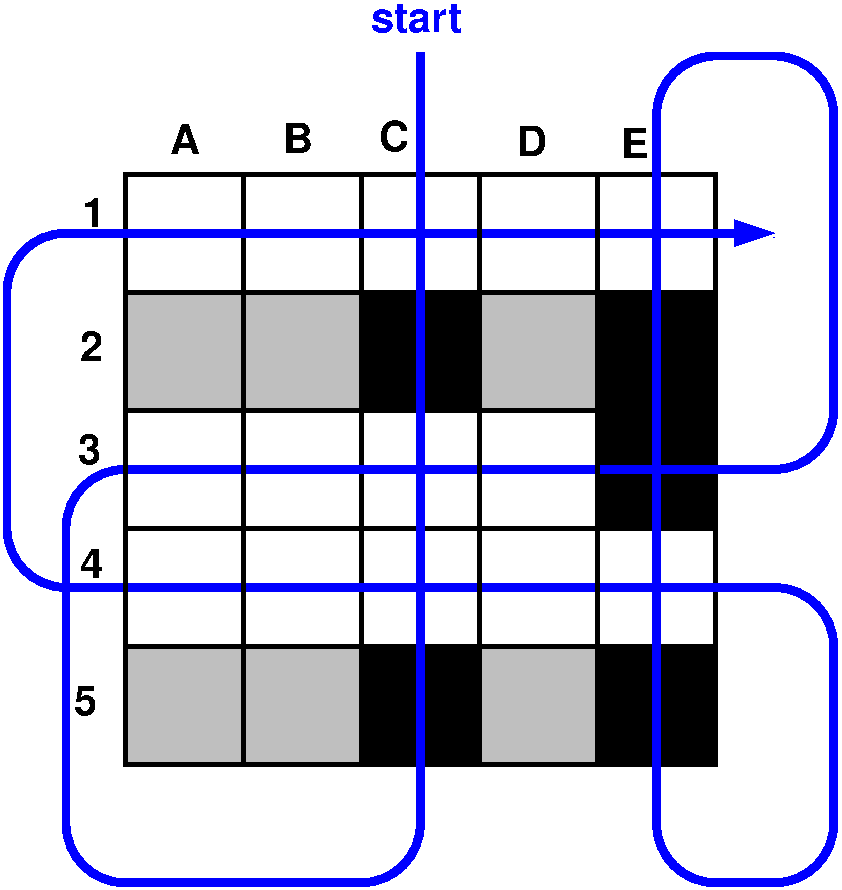
\includegraphics[width=5cm]{../skolkval/dentrottemalaren/problem_statement/golv.pdf}
\end{center}
\columnbreak
~\\ 
\emph{Pilen visar ett möjligt sätt att måla golvet i det andra körningsexemplet. Grå färg symboliserar omålade rutor.}
\vfill
\end{multicols}

\newpage
\specialsection*{Uppgift 5 -- Korta vokaler}

Att lösa algoritmproblem är svårt, men en sak som ofta är ännu svårare är att förbereda
testdatan. Ta problemet \textit{Arabiska} till exempel. Här har juryn lagt
många timmars intensivt arbete åt att konstruera mästerverk som \texttt{hej vad heter du}.

En fråga som dyker upp är: hur skapar man textsträngar som inte innehåller några korta vokaler?
Om du läste uppgiften \textit{Arabiska} så kanske du kommer ihåg att en kort vokal är en
vokal som följs av minst två konsonanter. I ordet \texttt{tall} så är a:et en kort vokal, medan
ordet \texttt{potatis} inte har några korta vokaler. För enkelhets skull räknar vi  \textit{a, e, i, o, u, y} 
som vokaler i det här problemet.


Ett sätt att skapa ord som inte innehåller några korta vokaler är att utgå ifrån ett ord,
och sedan ta bort några bokstäver från det. Om vi utgår från \texttt{potatis} så 
skulle vi då kunna få \texttt{ptais} till exempel. Men om ordet istället blev \texttt{otats} så uppstod
tyvärr en kort vokal.


Din uppgift är att räkna antalet sätt att ta bort bokstäver från ett givet ord så att resultatet inte
innehåller några korta vokaler. Det är tillåtet att inte ta bort några bokstäver alls (i andra exemplet
så bidrar det med $1$ till svaret). Däremot är det inte tillåtet att ta bort alla bokstäver. Om samma ord
uppstår genom att ta bort olika mängder bokstäver, så räknas de separat (I första exemplet finns det två sätt
att få ordet \texttt{tal}, vi kan ta bort det första eller det andra \texttt{l}:et).

Skriv ett program som läser in ett ord $S$ med högst $50$ bokstäver. Ordet består bara av bokstäverna \texttt{a-z}. Programmet ska skriva ut ett heltal, antalet sätt att ta bort bokstäver så att ett ord utan korta vokaler bildas. Notera att svaret inte alltid får plats i ett $32$-bitars heltal i de senare testfallen.

\fe{Poängsättning:}\\
För testfall värda $1$ poäng gäller att alla bokstäver i $S$ är samma.\\
För testfall värda ytterligare $2$ poäng gäller att $S$ har högst $10$ bokstäver.


\vspace{1cm}

\fe{Körningsexempel 1}
\begin{verbatim}
Ord ? tall

Svar: 13
\end{verbatim}

\vspace{1cm}

\fe{Körningsexempel 2}
\begin{verbatim}
Ord ? potatis

Svar: 107
\end{verbatim}


\newpage
\specialsection*{Uppgift 6 -- Bergskedja}


\noindent
Torunn bor i ett bergigt bostadsområde som består av ett $n \times m$-rutnät med en tomt i varje ruta.
Torunn bor på rutan längst upp till vänster i rutnätet.
Tyvärr har en extra jobbig hyresgäst nyligen flyttat in, så Torunn har bestämt sig för att sälja sin bostad och flytta någon annanstans.
Först måste hon dock ta reda på hur mycket bostaden är värd.

Varje ruta i rutnätet har en höjd. Alla höjder är olika, så låt oss för enkelhets skull anta att höjderna är $1, 2, 3, \cdots, n\cdot m$.
Tomter med högre höjd är värda mer på bostadsmarknaden, så Torunn vill ta reda på höjden på sin tomt. Hon har därför gått runt till varje ruta i rutnätet och kollat hur många angränsande rutor som är lägre.
En ruta anses vara angränsande om den delar en sida (rutor som inte ligger längs en kant har alltså $4$ angränsande rutor).

Skriv ett program som, givet informationen Torunn samlade in, hittar minsta och största möjliga höjd för rutan i övre vänstra hörnet.

Programmet ska läsa in två heltal $n$ och $m$ ($1 \leq n,m \leq 8$), antalet rader och kolumner i
rutnätet. Därefter ska det läsa in $n$ rader vardera innehållande en sträng med längden $m$. Detta rutnät utgör informationen
som Torunn samlade in, varje siffra motsvarar alltså antalet angränsande rutor som är lägre än rutan som
siffran står i. Det är garanterat att det finns minst ett sätt att tilldela höjderna 
$1, 2, \cdots, n\cdot m$ till rutorna så att den insamlade informationen är korrekt. Notera att värdena
som samlats in alltid kommer vara mellan $0$ och $4$.

Programmet ska skriva ut två heltal, den minsta och den största möjliga höjden på rutan i övre vänstra hörnet.

\fe{Poängsättning}\\
För ett poäng gäller att $n = 1$.\\
För ytterligare 1 poäng gäller att $n = m = 3$.\\
För ytterligare 1 poäng gäller att $n = m = 4$.\\

\vspace{0.5cm}

\setlength\columnsep{30pt}
\begin{multicols}{2}

\fe{Körningsexempel 1}
\begin{verbatim}
n ? 2
m ? 3
Rad 1 ? 122
Rad 2 ? 101

Svar: 3 4
\end{verbatim}

\vspace{0.5cm}
\fe{Körningsexempel 2}
\begin{verbatim}
n ? 1
m ? 4
Rad 1 ? 0111

Svar: 1 1
\end{verbatim}

\vfill\columnbreak
\begin{center}
  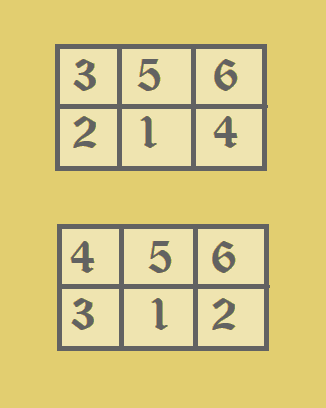
\includegraphics[width=5cm]{../skolkval/bergskedja/problem_statement/berg_sample}\\
  \emph{Två möjliga höjdkartor som stämmer överens med körningsexempel $1$.}
\end{center}
\vfill
\end{multicols}



\end{document}

